\documentclass[twocolumn]{article}
\usepackage{authblk}
\usepackage{amsmath}
\usepackage{graphicx}
\usepackage{textcomp}
\usepackage{color}
\usepackage{blindtext}
\usepackage{listings}
\usepackage{abstract}
\lstset{language=Matlab}

\begin{document}
\title{LAB ROTATION REPORT \\ }
\date{01.04.2013}
\author[1]{\c{S}eyma BAYRAK\thanks{seyma.bayrak@st.ovgu.de}}
\affil[1]{\footnotesize  Otto von Guericke University of Magdeburg}
\maketitle
\newpage

\twocolumn[
\begin{@twocolumnfalse}
\begin{abstract}

ABSC
\\ 

\end{abstract}

\end{@twocolumnfalse}  ]
 

 \section{Introduction}


 \section{Theoretical Background}
Wilson-Cowan model introduces a solution to the derivative of a time dependent activity $u(t)$ by consideriong an external input $s(t)$ in addition to Gaussian white noise $\xi(t)$ as the following;

\begin{equation}
 \tau\dot{u}(t)=-u+\Phi(u,s)+\sigma\sqrt{\tau}\xi(t)
\end{equation}
\begin{equation*}
\rightarrow du(t)=-\frac{u}{\tau}dt+\frac{1}{\tau}\Phi(u,s)dt+\frac{\sigma}{\sqrt{\tau}}n(t)\sqrt{dt} 
\end{equation*}
where $\tau$ is the time constant, $\sigma$ is the amplitute of the Gaussian white noise, and $\Phi(u,s)$ is the \textit{generalized logistic function (GLF)} depending on the input $s(t)$.

\subsection{GLF}
In order to compute the activity $u(t)$ iteratively as Wilson-Cowan model suggests, GLF must be defined properly. The generalized logistic function (GLF) is expressed below, as suggesed by Maurizio. 

\begin{equation}
 \Phi(x)=(1+e^{-\beta x+\alpha})^{-1/\nu}
\end{equation}

Either eqaution 1 or 2 are not trivial to fit the computed or expected activity $u(t)$ ideally to the experimental result plots, since they both depend on many parameters such that $\tau$, $\sigma$, $\beta$, $\alpha$ and $\nu$. Those parameters must be chosen well reasonably. My lab rotation has actually started with the analysis of GLF function, how it looks like with different parameters. This subsection reflects the shape of GLF function under change of its parameters.

 
\subsubsection{Inflection Point and $~ \nu$}
Inflection point on a curve is basically defined as the point at which curvature changes sign, or the second derivative of the curve equals to zero. When equation 2 is reduced to the form of $\Phi''(x)=0$, the inflection point's parameters seem to be as in the following:
\begin{equation*}
 x_{inf}=\dfrac{\alpha-ln\nu}{\beta},   \;\;\;\;\;\;        y_{inf}=(1+\nu)^{-1/\nu}
\end{equation*}

Once the $y_{inf}$ is chosen, the $\nu$ parameter can be calculated. A more sophisticated explanation could be more like that, once it is determined when the curvature of GLF changes its sign, then $\nu$ is found out automatically.  

\begin{center}
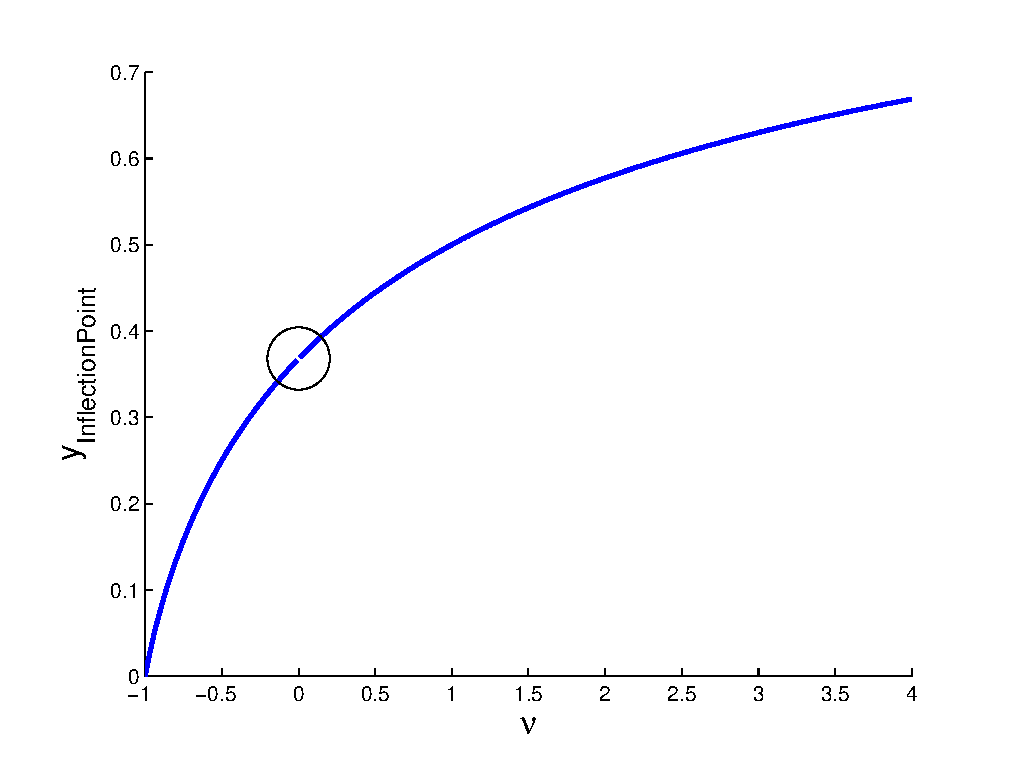
\includegraphics[width=80mm,height=60mm]{inflection_point.eps} 
   \begin{footnotesize} Figure 1 : The relation between the parameter $\nu$ and the inflection point on y axis. As long as $\nu$ is less than 0, then y is smaller than 1/e, otherwise y is greater than 1/e. Note that the singularity at 0.  \end{footnotesize}
\end{center}

What about the slope just at the inflection point? The slope is found by taking first derivative of GLF given by equation 2. 
\begin{equation*}
\Phi'(x)=y'_{inf}=\beta(1+\nu)^{-1-1/\nu}   
\end{equation*}

\subsubsection{Bisection Point and $\beta$, $\alpha$}
The bisection point divides GLF into two equal parts. In case GLF is restricted as having values between 0 and 1, the bisection point of it is $\Phi(x)=0.5=y_{1/2}$. Equation 2 yields up $x_{1/2}$ as stated below.
\begin{equation*}
 x_{1/2}=\dfrac{\alpha-ln(2^{\nu}-1)}{\beta}
\end{equation*}
Moreover, the slope of GLF function exactly at that bisection point can be expressed by in terms of the parameters. 
\begin{equation*}
 y'_{1/2}=\dfrac{\beta}{2\nu}(1-2^{-v})
\end{equation*}

\subsubsection{Start from Inflection and Plot GLF}
Let us summarize step by step how to eliminate GLF: assign values to inflection points $y_{inf}$, $x_{inf}$ and slope at inflection $y'_{inf}$. Now, the $\nu$ value can be calculated, (e.g. \textit{fsolve} command on MATLAB), $\beta$ can be found through the formula giving $y'_{inf}$ , and $\alpha$ is derived from the formula expresses $x_{inf}$.

\begin{itemize}
\item $\nu=@fsolve((\nu) \;\;\; (1+\nu)^{-1/\nu}-y_{inf})$
\item $\beta=y'_{inf}.(1+\nu)^{1+1/\nu}$
\item $\alpha=\beta.x_{inf}+ln\nu$
\end{itemize}

Let us plot two GLF functions, the assigned parameters are the as the following: for the first GLF (dashed red line); $y_{inf}=0.25$, $x_{inf}=0.5$, $y'_{inf}=1.5$, for the second GLF (solid red line); $y_{inf}=0.75$, $x_{inf}=0.5$, $y'_{inf}=1.5$.  

\begin{center}
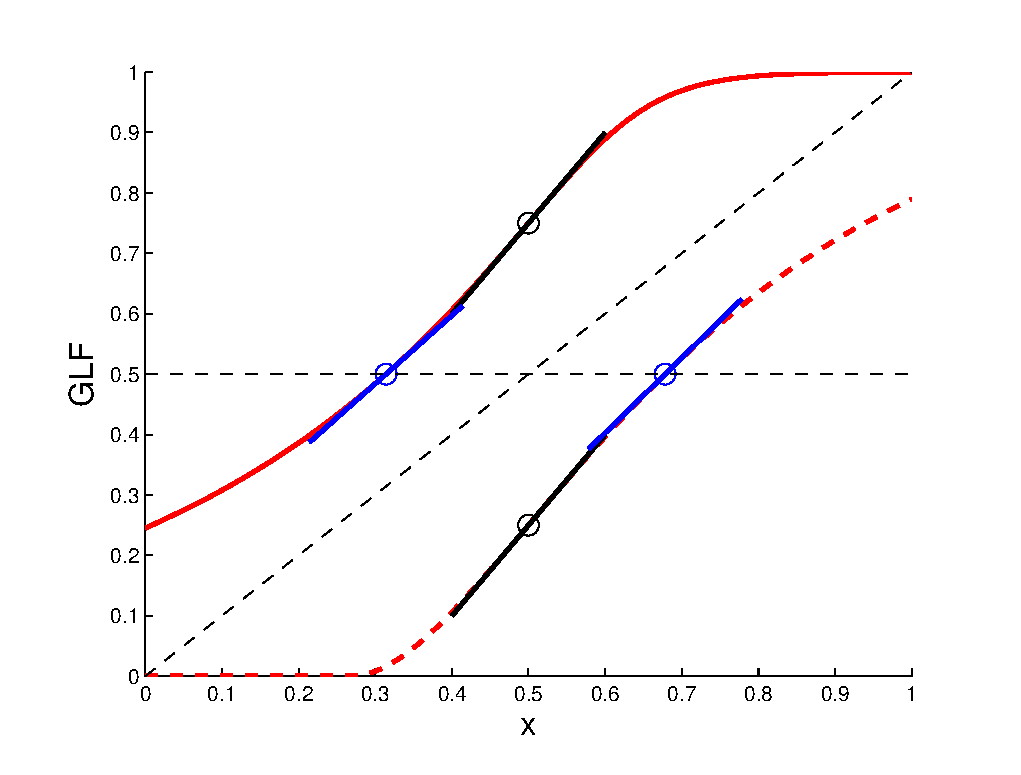
\includegraphics[width=80mm,height=60mm]{glf_first.eps} 
   \begin{footnotesize} Figure 2 : The short-solid black lines indicate the slope around inflection points, whereas the blue lines indicate that of bisection points. Note that when $y_{inf}$ is smaller than 1/e, the parameter $\nu$ is smaller than 0.  \end{footnotesize}
\end{center}

\subsubsection{Different $\alpha$ values and GLF }

Now, GLF can be thought more sophisticated as $\Phi(x,s)$ rather than $\Phi(x)$. If $s$ is assumed to be an external input such as a stimuli, and if $\alpha$ is defined as depending on $s$, it is better to express it in a form such that $\Phi(x,s)$. Let us define a linearly changing stimuli  $s=[0 0.25 0.50 0.75 1]$ and make $\alpha$ depended on it:
\begin{equation}
 \alpha=\alpha_0+(\alpha_1-\alpha_0).s
\end{equation}
where $\alpha_1$ and $\alpha_0$ are constants. The following GLF function is elliminated. 

\begin{center}
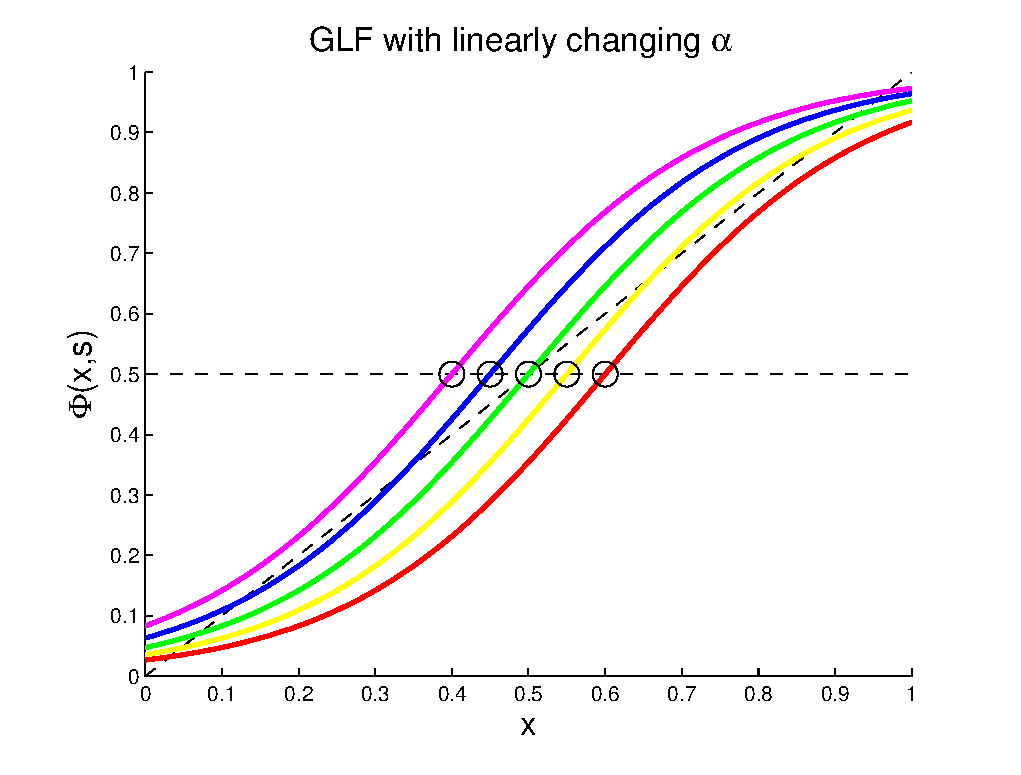
\includegraphics[width=80mm,height=60mm]{linear_alpha.eps} 
   \begin{footnotesize} Figure 3 : As long as $\alpha$ changes, the GLF shiftes to the left around the bisection point. Here, $y_{inf}=0.5$, $y'_{inf}=1.5$, $\alpha$ is given, and the other parameters necessary for GLF are all calculated through the similar steps indicated in section 2.1.3. \end{footnotesize}
\end{center}

\subsubsection{Steady State Points of GLF}
Steady states point are the points where a bifurcation is observed on the GLF function. In other words, steady state points are assumed to be locating on where the sigmoidal-like GLF functions intersects with $x=y$ line. The trick is to assume that $\Phi(x,s) \approx x$ and then let MATLAB find those points with \textit{fsolve} command.
 
\begin{center}
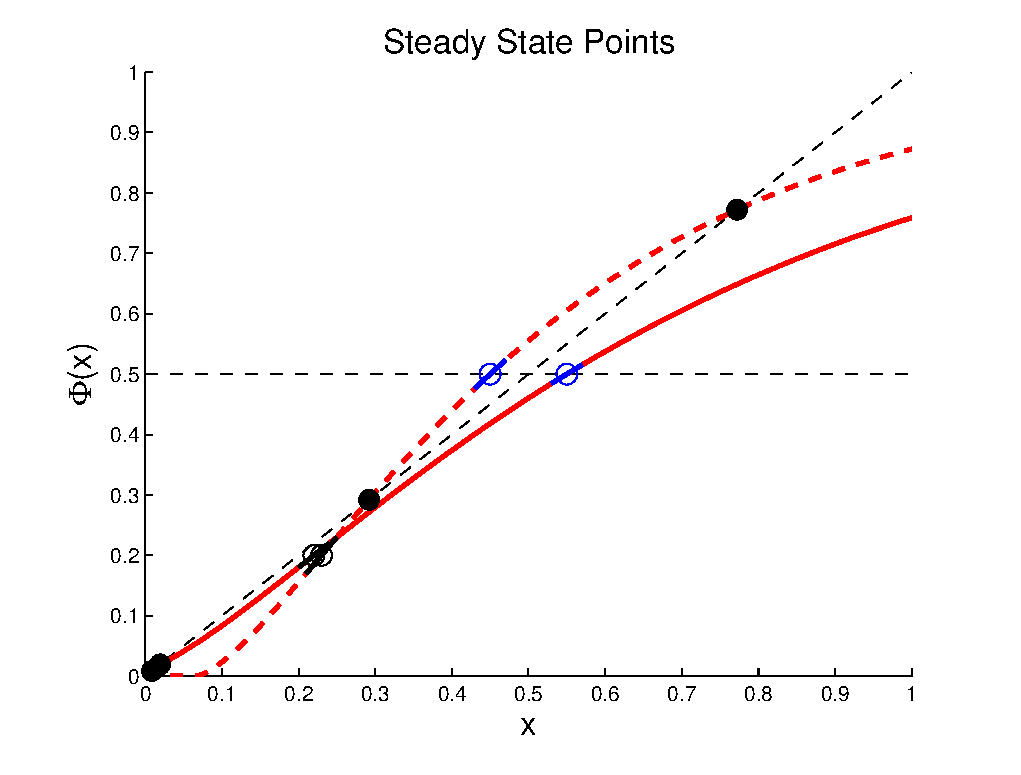
\includegraphics[width=80mm,height=60mm]{steady_state.eps} 
   \begin{footnotesize} Figure 4 : Two GLF with steady state points as indicated as large-black filled up circles. Here, the assigned parameters for the solid line GLF: $y_{inf1}=0.2$, $y'_{inf1}=1.0$, $x_{1/2}=0.55$ and $y_{1/2}=0.5$, for the dashed line GLF:$y_{inf1}=0.2$, $y'_{inf1}=1.0$, $x_{1/2}=0.45$ and $y_{1/2}=0.5$.  \end{footnotesize}
\end{center}

 One single GLF function (with one $\alpha$ parameter) can have maximum three steady state point; those can be categorized as 'high - middle - low steady state points'. Let us now assume that the external input $s$ is changing linearly between 0.1 and 0.9. Therefore the s depended $\alpha$ also changes according to equation 3. The figure below indicates all possible steady state points of many GLF which has different $s$ or in other words different $\alpha$ value each time. 

\begin{center}
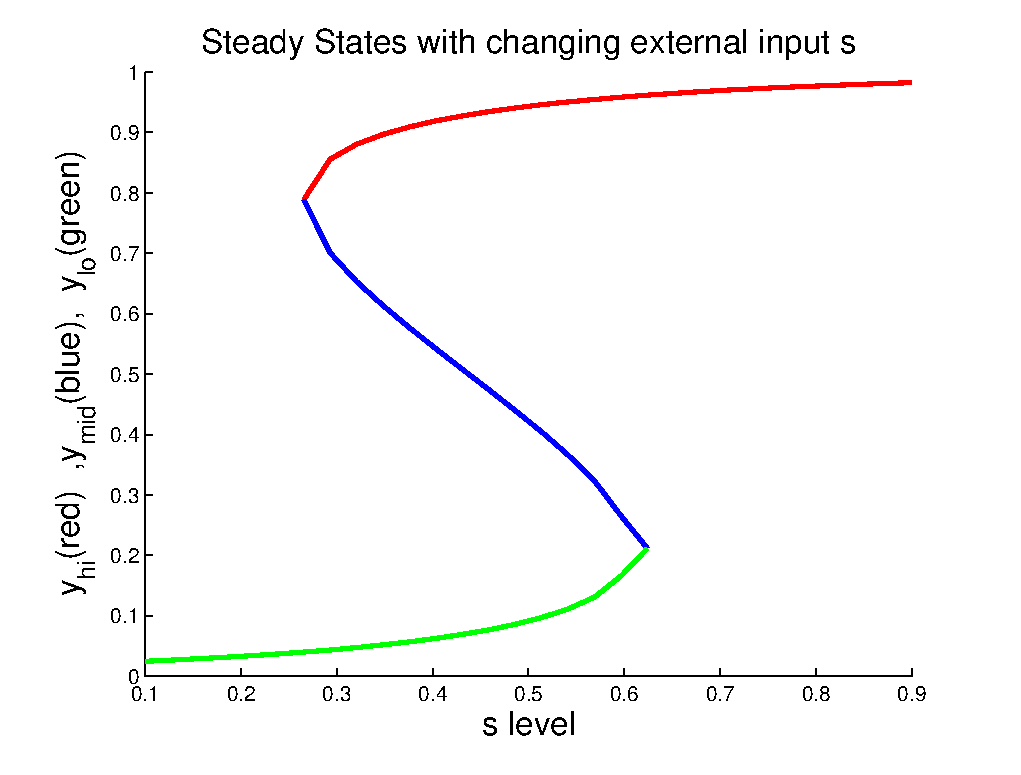
\includegraphics[width=80mm,height=60mm]{s_vs_steadystate.eps} 
   \begin{footnotesize} Figure 5 : Steady state points of different GLF functions corresponding to given $s$ values on x axis. Note that at each s value, there could be maximum three steady state points which could be in high - middle - low transition areas. \end{footnotesize}
\end{center}


\subsection{Wilson Cowan Model with Step Input}
After analysing GLF, it is yet simpler to determine the activity $x(t)$ with Wilson-Cowan model. However, GLF is defined as depending on an external parameter called $s$. In fact, this parameter represents the ``coherence'' of the rotating dots in my experiment, so it is an input related to the stimulus. We would like to have very randomly moving dots with 0 coherence during the beginning of stimuli time, then increase coherence up to 100 \% and then reduce it back to an intermediate level around 40 \%. The corresponding $s$ graph is shown below. 

 \begin{center}
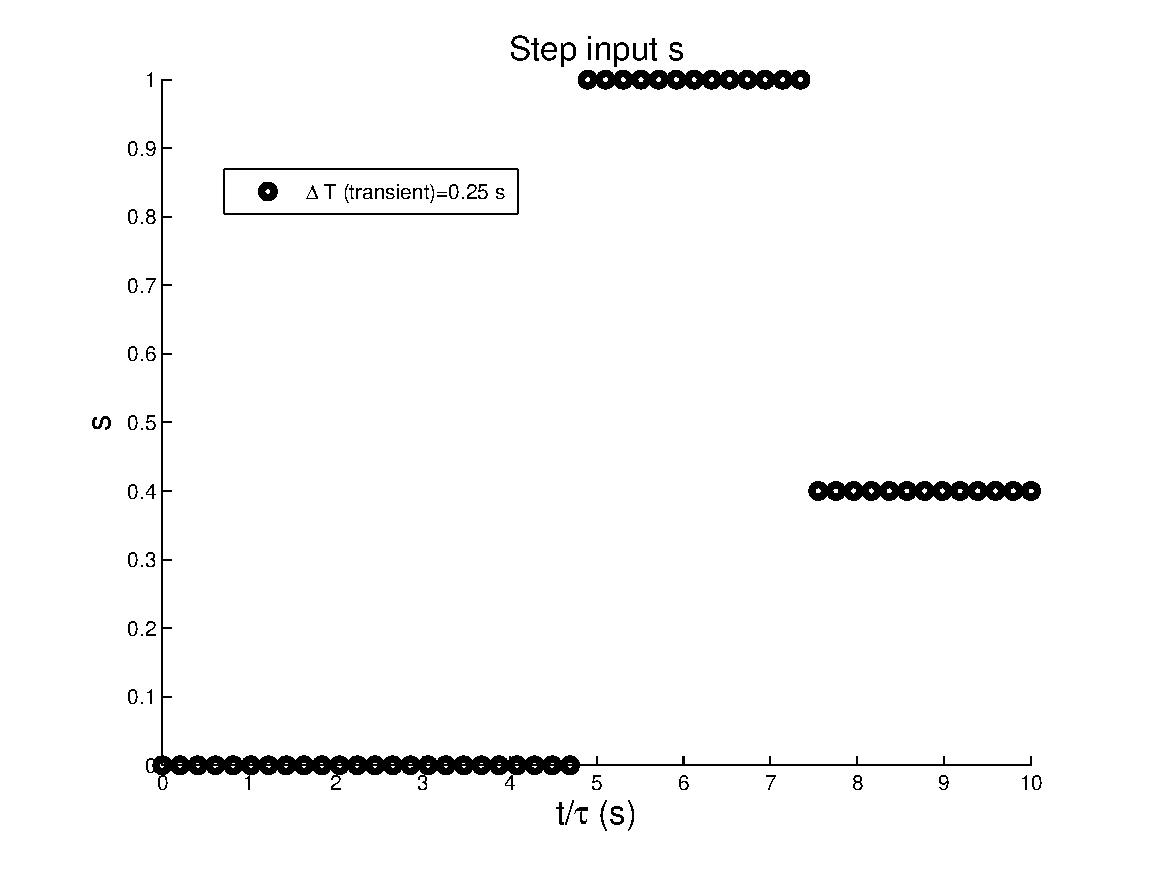
\includegraphics[width=80mm,height=60mm]{step_s.eps} 
   \begin{footnotesize} Figure 6 : A step input level changing in time (divided by time constant on the x axis).  Transient time corresponds to width of maximum coherence in terms of duration. \end{footnotesize}
\end{center}

The well-defined parameters are now inserted into GLF, inclusively the parameter $\alpha$ with the dependence of the step input just shown above. The activity $x(t)$ is calculated by the numerical inegration of Equation 1 as Wilson-Cowan model suggested previously. The initial point of the activity $x_0$ is chosen to be 0, this corresponds to "no perception at the beginning" in my experiment.

 \begin{center}
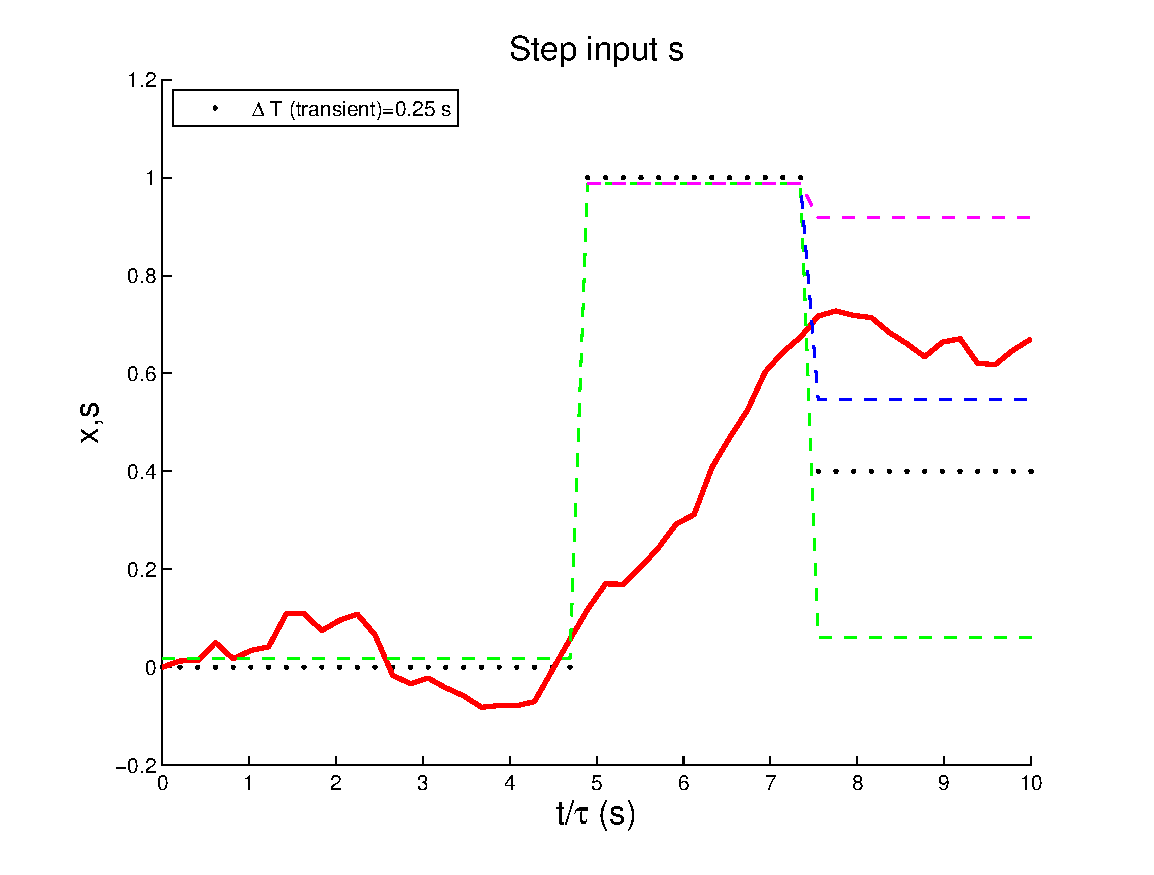
\includegraphics[width=80mm,height=60mm]{my_WC.eps} 
   \begin{footnotesize} Figure 7 : The activit $x$ is reflected as the red line above, black dots represent the step input $s$, and dashed lines stand for the steady state points of GLF for each $s$ value, green for the low steady state points, blue for intermediate transition levels, and magenta for high steady state points.  \end{footnotesize}
\end{center}

\subsection{Activity Probability of $s$ with Different Transient Values}
The whole concern is actually to figure out where the activity $x(t)$ ends up. The activity itself is the theoretical model of the perception of the "observer". The initial value $x_0$ is already chosen to be 0, but the interested value is what $x(t)$ equals to after the total time duration of the model step stimuli. When the last value of $x(t)$ is greater than 0.5, it is assumed that the activity is successful, otherwise failed. To explain it more understable, let us use Figure 7, there the activity (red curve) ends up somewhere around greater than 0.5, so it is a successful or correct activity.

Since $x(t)$ depends on a Gaussian white noise meaning a series of randomness, the correctness of activity needs to be calculated by a  statistical approach. In my program, I run the program 200 times for each step input coherence $s$ and then got a fraction of successful results of activity overall 200 trials as the following:
\begin{equation}
 P_{correct}=\dfrac{number \;\;\;of\;\;\;correct\;\;\;trials}{number\;\;\;of\;\;\;total\;\;\;trials}
\end{equation}

The last step of my theoretical anaylsis is to create $s$ with different transient durations. The 100 \% coherence level duration is changed linearly between 0.1 and 0.9 seconds. Then, Wilson-Cowan model is applied to find out the $x$, and $P_{correct}$ is eliminated.

 \begin{center}
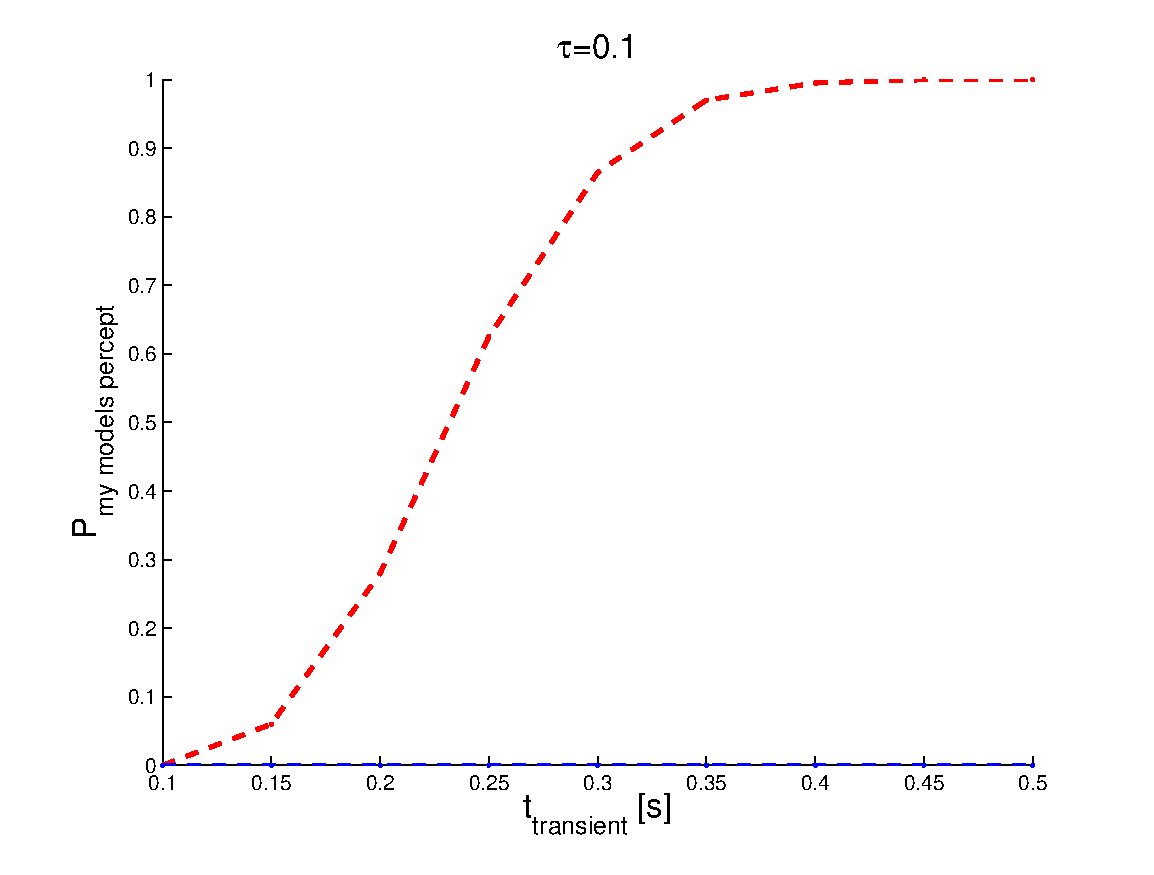
\includegraphics[width=80mm,height=60mm]{my_P_correct.eps} 
   \begin{footnotesize} Figure 8 : The red-dashed line represents the probability of correct activities corresponding to transient durations. The blue-dashed line is the same procedure repeated for the $s$ having no transient duration, it is assumed to be a "baseline".  \end{footnotesize}
\end{center}

\section{Experimental Part}




\end{document}
